\chapter{Architecture Diagram}

\section{Description}
The system will rely on an event-based architecture. As shown in the architecture digram (Figure \ref{fig:architecture}), the arrows show the flow of data between the different components of the system. The doorbell button triggers an event that goes to the Raspberry Pi Zero which acts as an announcer in this architecture. This event tells the announcer to broadcast the appropriate doorbell event to all types of devices currently registered in the system. The arrow going back into the doorbell is to offer feedback to the Visitor in order to confirm that the button was pressed and the event was broadcast to the Resident's devices. The arrow going to the Raspberry Pi Zero from the Home Network is to confirm that the devices received the broadcasted event.

\begin{figure}[h]
  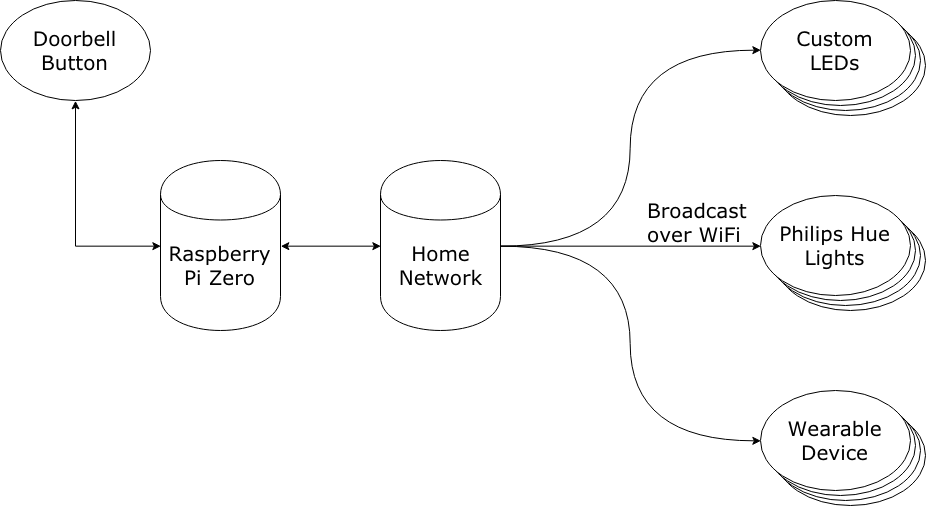
\includegraphics[width=0.8\textwidth]{Architecture-new.png}
  \centering
  \caption{Architecture Diagram}
  \label{fig:architecture}
\end{figure}